\section{Introduction}

\subsection{General Principles of Radiation Detection}

\subsubsection{Radiation Detection}

Measurements can either be done on
\begin{enumerate}
    \item Primary charges\\
    Gas detectors \& Semiconductor detectors
    \item Scintillation photons\\
    Scintillator detectors 
    \item Other\\
    Calorimeters, Cerenkov detectors, Combinations of 1. \& 2.
\end{enumerate}

\subsubsection{Signal Processing}
\begin{enumerate}
    \item Scope observation\\
    Direct observation of the Voltage-time plot on the oscilloscope 
    \item Counting\\
    With a certain voltage threshold, every peak higher than said threshold is recorded as a count
    \item Sorting by amplitude\\
    With a analog-to-digital (ADC) converter, different voltage values can be translated to a spectrum
\end{enumerate}
An ideal detector would have $V_{out}\propto i_{in}\propto E_{deposited}$

\subsubsection{Properties of Radiation Detection Systems}

\begin{enumerate}
    \item Sensitivity\\
    The ability to distinguish signal from noise
    \item Efficiency\\
    $\varepsilon=\frac{N_{det}}{N_{emit}}=\varepsilon_{geo}\times\varepsilon_{intrinsic}\times\varepsilon_{electronic}$\\
    $\varepsilon_{geo}=\frac{\Omega}{4\pi}$\\
    For thin, straight-on circular detectors,\\ $\varepsilon_{geo}=\frac{1}{4\pi}\int_0^{2\pi}d\phi\int_0^\alpha\sin\theta d\theta=\frac{1}{2}(-\cos\theta){|}_0^\alpha$\\
    $\cos\alpha=\frac{d}{\sqrt{d^a+a^2}}$(See figure~\ref{fig:geometry_efficiency_calc})\\
    $\Rightarrow\;\varepsilon_{geo}=\frac{1}{2}\left(1-\frac{d}{\sqrt{d^2+a^2}}\right)$
    \begin{figure}[ht]
    \centering
    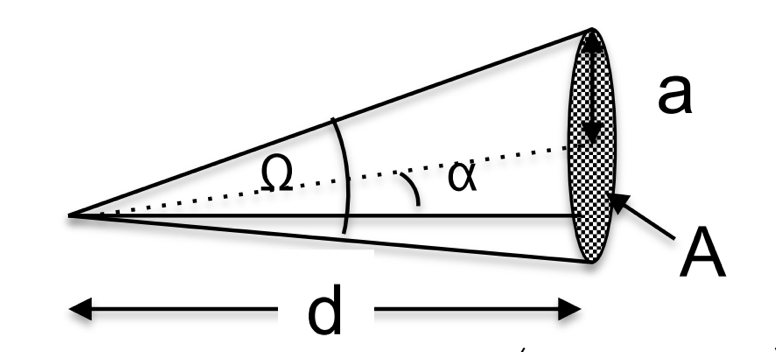
\includegraphics[width=0.3\textwidth]{images/efficiency_geo.png}
    \caption{Geometry efficiency calculation}
    \label{fig:geometry_efficiency_calc}
    \end{figure}
    \item Energy resolution\\
    Repeatability (peak width), not accuracy 
    \item Time resolution\\
    Ability to determine time of event
    \item Pulse-pair resolution\\
    Ability to resolve subsequent events
    \item Position resolution
\end{enumerate}
